\scanpage{11}
\uline{\unsure{Coh. prop. of maps in Cat}}

2) Immersions fermées et ouvertes

\uline{Propriétés cohomologiques}

\margin{not cofib. nor fib. (i.e. not closed imm nor open imm)}

\diagram{\begin{tikzcd}[column sep=large]
Y & \mathrm{Fib}(f) \arrow[l,"\unsure{f^b|f^\flat}","\text{fibration}"'] \arrow[r,bend right=35,"\rho_f"'] & X \arrow[l,"\unsure{\eta_f|H_f}\ \text{mono}"']
\end{tikzcd}}

(Fibers ${}_{b}\backslash X$ discretely cofibered /$X$)

\uline{but not yet} \uline{Serre}

(Serre cofibering) retraction

[fibers $Y_{/b}$ discr. fibered over $Y$]

\diagram{\begin{tikzcd}[column sep=large]
Y & \mathrm{Cofib}(f) \arrow[l,"\unsure{f^{b'}|f^{\flat\prime}}","\text{cofibration}"'] \arrow[r,bend right=35,"\rho'_f"'] & X \arrow[l,"\unsure{\eta'_f|H'_f}\ \text{mono}"']
\end{tikzcd}}

(fibers $X_{/b}$ discretely fibered /$X$)

\uline{but not yet Serre}

Serre \unsure{fibering} retraction

(fibers ${}_{b}\backslash Y$ discr. cofibered over $Y$)

but not

\figure{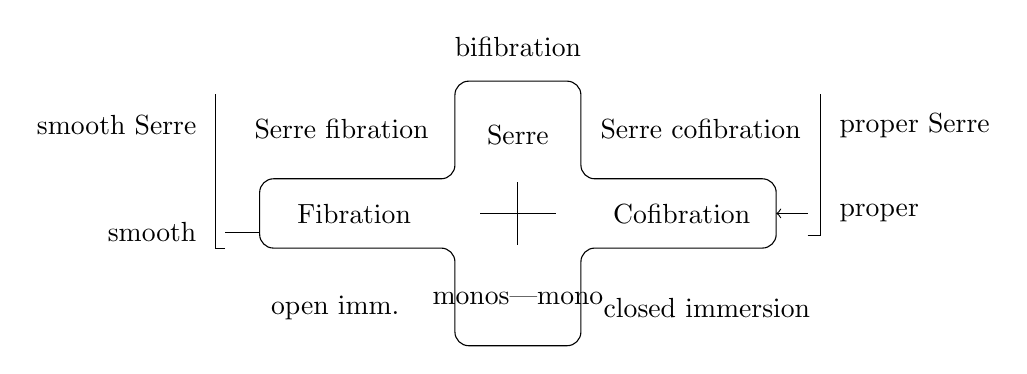
\begin{tikzpicture}[x=0.8cm,y=0.8cm]
\draw[rounded corners=5pt] (-1,2.1)--(1,2.1)--(1,.55)--(4.1,.55)--(4.1,-.55)--(1,-.55)--(1,-2.1)--(-1,-2.1)--(-1,-.55)--(-4.1,-.55)--(-4.1,.55)--(-1,.55)--cycle;
\draw (-.6,0)--(.6,0) (0,-.5)--(0,.5);
\node at (0,1.25) {Serre};
\node at (0,-1.35) {\unsure{monos|mono}};
\node at (-2.6,0) {Fibration};
\node at (2.6,0) {Cofibration};
\node at (0,2.65) {bifibration};
\node at (-2.8,1.35) {Serre fibration};
\node at (2.9,1.35) {Serre cofibration};
\node at (-2.9,-1.5) {open imm.};
\node at (3,-1.5) {closed immersion};
\draw (-4.1,-.3)--(-4.65,-.3) (-4.65,-.55)--(-4.8,-.55)--(-4.8,1.9);
\node[anchor=east] at (-4.95,1.4) {smooth Serre};
\node[anchor=east] at (-4.95,-.3) {smooth};
\draw[<-] (4.1,0)--(4.6,0);
\draw (4.6,-.35)--(4.8,-.35)--(4.8,1.9);
\node[anchor=west] at (4.95,1.4) {proper Serre};
\node[anchor=west] at (4.95,0) {proper};
\end{tikzpicture}}

\diagram{\begin{tikzcd}[column sep=large]
Y \arrow[r,hook,"\unsure{f^b|f^\flat}","\text{open imm}"'] & C(f) \arrow[r,"\lambda_f^{(\mathrm{op})}"] & X \arrow[l,bend left=35,"\sigma_f","\text{closed section}"']
\end{tikzcd}}

\diagram{\begin{tikzcd}[column sep=large]
Y \arrow[r,hook,"\unsure{f^{b'}|f^{\flat\prime}}\ \text{closed}","\text{imm}"'] & C'(f) \arrow[r,"\lambda'_f"] & X \arrow[l,bend left=35,"\sigma'_f","\text{open section}"']
\end{tikzcd}}

\diagram{\begin{tikzcd}[column sep=large]
Y \arrow[r,hook,"i_Y","\text{open imm}"'] & C(Y) \arrow[r,"\varepsilon_Y"] & e \arrow[l,bend left=35,"\text{closed section}"']
\end{tikzcd}}

($e$ \inserted{strict} final object)

\diagram{\begin{tikzcd}[column sep=large]
Y \arrow[r,hook,"i'_Y","\text{closed imm}"'] & C'(Y) \arrow[r,"\varepsilon'_Y"] & e \arrow[l,bend left=35,"\text{open section}"']
\end{tikzcd}}

($e$ strict initial object)

\[
C'(f)^\circ=C(f^\circ)\quad\text{i.e.}\quad C'(f)=C(f^\circ)^\circ
\]
\[
C'(Y)^\circ=C(Y^\circ)\quad\text{i.e.}\quad C'(Y)=C(Y^\circ)^\circ
\]
% archive foliation: 10
